\chapter{Analyse op 2 variabelen}
\label{ch:analyse2var}

In de vorige hoofdstukken hebben we telkens één variabele tegelijkertijd onderzocht. Vaak hebben onderzoeksvragen echter te maken met \emph{verbanden} (en dan vooral oorzakelijke) tussen variabelen. In dit hoofstuk gaan we hier verder op in.

Wanneer we een verband beschrijven tussen variabelen, onderscheiden we:

\begin{itemize}
  \item De \emph{afhankelijke variabele}\index{variabele!afhankelijke}, waarover we een voorspelling willen doen;
  \item De \emph{onafhankelijke variabele}\index{variabele!onafhankelijke}, op basis van dewelke we de voorspelling doen.
\end{itemize}

Als de onafhankelijke variabele op een bepaalde manier verandert, verwachten we dat de waarde van de afhankelijke variabele op een voorspelbare manier mee verandert.

\begin{example}
  Een voorbeeld waarbij verbanden kunnen gevonden tussen variabelen vind je bijvoorbeeld bij Ant Colony Optimization (ACO). Dit is een techniek die gebruikt wordt in verschillende computationele problemen. Men baseert zich hier op hoe mieren voedsel zoeken en  vinden en dat communiceren aan de groep. Mieren verspreiden feromonen als ze op pad gaan op zoek naar eten. Hoe langer het pad, hoe minder feromonen het pad zal bevatten, hoe korter het pad, hoe groter de kans dat er een grote concentratie aan feromonen te vinden is. Mieren worden aangetrokken door deze feromonen en zullen dus proberen de meest bewandelde paden te gebruiken om naar een bepaalde voedselbron te gaan. Nu kan je onderzoeken of de tijd voor het vinden van een pad, afhangt van een aantal variabelen:

  \begin{itemize}
    \item De mate waarin feromonen verspreid worden
    \item De mate waarin een feromoon verdwijnt
    \item Het aantal obstakels tussen het nest en de voedselbron
    \item De vorm van de obstakels tussen nest en voedselbron (vinden ze sneller het pad indien er geen hoeken aan de obstakels zijn bv.)
  \end{itemize}
\end{example}

Om een vergelijking te maken kunnen we \begin{inparaenum}[(i)]
\item de bekende statistieken zoals gemiddelde e.a. berekenen en analyseren of \item grafische voorstellingen maken van deze statistieken. \end{inparaenum}

Welke soort van grafieken we kunnen gebruiken hangt af van het meetniveau:
@
\begin{itemize}
  \item Interval of ratio:

    \begin{itemize}
      \item Staafdiagram van de gemiddelden
      \item Boxplot per groep
    \end{itemize}
  \item Ordinaal of nominaal

    \begin{itemize}
      \item Kruistabel
      \item Geclusterd staafdiagram
      \item Rependiagram
    \end{itemize}
\end{itemize}

Bij de vraag of er samenhang is tussen twee variabelen kunnen we volgende grafieken/statistieken gebruiken:

\begin{itemize}
  \item Nominaal x Nominaal:

    \begin{itemize}
      \item Kruistabel met Cramér's V
    \end{itemize}
  \item Ordinaal x Ordinaal
    \begin{itemize}
      \item Geclusterd staafdiagram
      \item Rependiagram
    \end{itemize}
  \item Ratio x Ratio

    \begin{itemize}
      \item Spreidingsdiagram
      \item Regressie en correlatie met correlatiecoëfficiënt.
    \end{itemize}
\end{itemize}

\section{Kruistabellen en Cramér's V}

\begin{definition}[Kruistabel]
  In een kruistabel\index{kruistabel} (zie bv.~Figuur~\ref{tab:kruistabel0}) worden de frequenties van twee variabelen samengevat.
  
  Elke cel van de laatste kolom bevat de som van de overeenkomstige rij en elke cel van de laatste rij bevat de som van de overeenkomstige kolom. Dit worden de \emph{marginale totalen}\index{totaal!marginaal}\index{marginaal totaal} genoemd.
\end{definition}

In R kan je een kruistabel (Eng.: \emph{contingency table} of \emph{cross table}) opstellen met de functie \texttt{table}. Een voorbeeld i.v.m.~de oefening over Android persistentietypes (zie Oefening~\ref{oef:casus-akin2016-1var}):

\begin{lstlisting}
> table(Datahoeveelheid, PeristentieType)
        PersistentieType
DataHoeveelheid GreenDAO Realm Sharedpreferences SQLLite
Large                 30    30                 0      30
Medium                30    30                 0      30
Small                 30    30                30      30
\end{lstlisting}

\begin{table} \centering
  \begin{tabular}{@{}rrrr}
    \toprule
                & Vrouw & Man & Totaal \\ \midrule
           Goed &     9 &   8 &     17 \\
      Voldoende &     8 &  10 &     18 \\
    Onvoldoende &     5 &   5 &     10 \\
         Slecht &     0 &   4 &      4 \\
         Totaal &    22 &  27 &     49 \\ \bottomrule
  \end{tabular}
  \caption{Een kruistabel voor de waardering door mannen en vrouwen van een bepaald assortiment producten.}
  \label{tab:kruistabel0}
\end{table}

In een gewone kruistabel kunnen we geen directe conclusies trekken, aangezien het analyseren of er samenhang bestaat tussen variabelen niet goed gaat op basis van de celfrequenties. Niet alle metingen zijn even groot! Daarom moeten we percenteren. Nog even snel de regel van percenteren:

\begin{itemize}
  \item Om te weten hoeveel percent $x$ is van $y$, deel je $x$ door $y$ en vermenigvuldig je met 100: $perc = 100 \times \frac{x}{y}$.
  \item Om te weten hoeveel $x$ \% is van $y$ : $ \frac{x \times y}{100}$
\end{itemize}

\begin{example}
  \label{vb:kruistabel}
  In Tabel~\ref{tab:kruistabel0} vinden we de data waar er gekeken wordt naar het verschil in waardering van een assortiment tussen mannen en vrouwen. We percenteren per geslacht en vinden bijvoorbeeld dat 41\% van de vrouwen een waardering goed heeft (zie Tabel~\ref{tab:kruistabel1}). Nu kunnen we ons de vraag stellen of de waarderingskeuze afhangt van het geslacht van de persoon.
\end{example}

In ons voorbeeld kunnen we besluiten dat 30\% van de mannen tevreden is en 15\% van de mannen ontevreden. Maar hoe goed is die samenhang tussen de verschillende variabelen (geslacht en tevredenheid)? Dat kunnen we bepalen aan de hand van Cramér's V. Voordat we die definitie kunnen geven, moeten we echter eerst de waarde $\chi^2$ introduceren.

\begin{table} \centering
  \begin{tabular}{@{}rrrrrrr@{}} \toprule
    & Vrouw & Man & Totaal & Vrouw \% & Man\%   & Totaal  \\ \midrule
    Goed        & 9     & 8   & 17     & 41\%  & 30\% & 35\% \\
    Voldoende   & 8     & 10  & 18     & 36\%  & 37\%    & 37\% \\
    Onvoldoende & 5     & 5   & 10     & 23\%  & 18\% & 20\% \\
    Slecht      & 0     & 4   & 4      & 0\%      & 15\% & 8\%  \\
    Totaal      & 22    & 27  & 49     & 100\%    & 100\%   & 100\%   \\
    \bottomrule
  \end{tabular}
  \caption{De kruistabel waarbij we de waarden gepercenteerd hebben.}
  \label{tab:kruistabel1}
\end{table}

\section{\texorpdfstring{$\chi^{2}$}{chi-kwadraat} test voor associatie}
\index{$\chi^{2}$waarde}

De $\chi^{2}$ (\emph{chi-kwadraat}) waarde is een grootheid die gebruikt wordt om te bepalen of er een significant verband bestaat tussen twee variabelen. Meer hierover volgt later in Hoofdstuk~\ref{ch:chikwadraat}. De berekening ervan leggen we alvast hier uit.

\begin{enumerate}
  \item Stel de kruistabel op samen met marginale totalen (zie tabel \ref{tab:kruistabel1}).
  \item Stel voor elke cel een schatter op voor de theoretische kans om in die cel te geraken. Deze schatter kan je bereken als volgt: (kans op in de rij van deze cel te komen) $\times$ (kans om in de kolom van de cel te komen). In het voorbeeld is dit dus voor cel$_{1,2}$:
  
  \[P[rij_{1}] \times P[kolom_{2}] = \frac{17}{49} \times \frac{27}{49} = 0.191170346 \]
  Algemeen kan je dus stellen dat de verwachte theoretische waarde $e$ als volgt kan berekend worden:

  \begin{equation}
    e = (\frac{rijtotaal}{n} \times \frac{kolomtotaal}{n}) \times n = \frac{rijtotaal \times kolomtotaal}{n}
  \end{equation}

  Met:

  \begin{itemize}
    \item $e$ verwachte waarde bij onafhankelijkheid
    \item $rijtotaal$ totaal van de rij van de betreffende cel
    \item $kolomtotaal$ totaal van de kolom van de betreffende cel
  \end{itemize}

  Voor cel$_{1,2}$ is dit dus 9.36.
  
  \item Dan bereken je het verschil tussen geobserveerde (notatie $a$) en verwachte frequentie ($e$). (Zie tabel \ref{tab:kruistabel2})
  
  \item De laatste stap houdt in dat we een berekening gaan maken voor de maat van afwijking voor elke cel. Opnieuw gaan we hier een kwadraat nemen om het teken kwijt te spelen. We gaan ook de afwijking delen door de verwachte theoretische waarde om hen relatief even belangrijk te maken. Bijvoorbeeld: een afwijking van 5 op een verwachte frequentie van 20 is groter dan bv. een afwijking op een verwachte waarde van 200. Dit geeft dan volgende berekening (zie Tabel~\ref{tab:kruistabel3}):
  
  \begin{equation}
    \frac{(a-e)^{2}}{e}
  \end{equation}
  
  \item Deze gekwadrateerde deviaties gaan we dan optellen en vormt de $\chi^{2}$ \footnote{Let op dat er afgerond wordt.}
  
  \begin{equation}
    \chi^{2} = \sum \frac{(a-e)^{2}}{e}
  \end{equation}
\end{enumerate}

\begin{table} \centering
  \begin{tabular}{@{}rrrrrrr@{}} \toprule
    & Vrouw & Man & Totaal & Vrouw \% & Man\%   & Totaal  \\ \midrule
    Goed        & $9 -\textcolor{red}{7.63}$     & $8 - \textcolor{red}{9.36}$   & $17$     & $41$\%  & $30$\% & $35$\% \\
    Voldoende   & $8 - \textcolor{red}{8.08}$   & $10 - \textcolor{red}{9.91}$  & $18$     & $36$\%  & $37$\%    & $37$\% \\
    Onvoldoende & $5 - \textcolor{red}{4.48}$    & $5 - \textcolor{red}{5.51}$  & $10$     & $23$\%  & $18$\% & $20$\% \\
    Slecht      & $0 - \textcolor{red}{1.79}$    & $4 - \textcolor{red}{2.20}$  & $4$      & $0$\%      & $15$\% & $8$\%  \\
    Totaal      & $22$    & $27$  & $49$     & $100$\%    & $100$\%   & $100$\%   \\
    \bottomrule
  \end{tabular}
  \caption{De kruistabel waarbij we de schatter $e$  (hetgeen we verwachten bij geen samenhang) bepaald hebben voor elke cel en die aftrekken van de geobserveerde waarde.}
  \label{tab:kruistabel2}
\end{table}

\begin{table} \centering
  \begin{tabular}{@{}rrrrrrr@{}} \toprule
    & Vrouw                   & Man                     & Totaal & Vrouw \% & Man\%   & Totaal  \\ \midrule
    Goed        & $\textcolor{blue}{0.2}$ & $\textcolor{blue}{0.2}$ & $17$   & $41$\%   & $30$\%  & $35$\% \\
    Voldoende   & $\textcolor{blue}{0}$   & $\textcolor{blue}{0}$   & $18$   & $36$\%   & $37$\%  & $37$\% \\
    Onvoldoende & $\textcolor{blue}{0.1}$ & $\textcolor{blue}{0}$   & $10$   & $23$\%   & $18$\%  & $20$\% \\
    Slecht      & $\textcolor{blue}{1.8}$ & $\textcolor{blue}{1.5}$ & $4$    & $0$\%    & $15$\%  & $8$\%  \\
    Totaal      & $22$                    & $27$                    & $49$   & $100$\%  & $100$\% & $100$\%   \\
    \bottomrule
  \end{tabular}
  \caption{De kruistabel waarbij we het verschil gekwadrateerd en genormeerd hebben.}
  \label{tab:kruistabel3}
\end{table}

Met deze statistiek kunnen de waarde Cramér's V\index{Cramér's V} berekenen:

\begin{definition}[Cramér's V]
  \begin{equation}
    V = \sqrt{\frac{\chi^{2}}{n(k-1)}}
    \label{eq:Craemer}
  \end{equation}
  met
  \begin{itemize}
    \item $\chi^{2}$ de berekende chi-kwadraatwaarde.
    \item $n$ het aantal waarnemingen.
    \item $k$ = de kleinste waarde van het aantal kolommen of het aantal rijen van de tabel.
  \end{itemize}

\end{definition}

Cramér's V is de $\chi^{2}$, gecorrigeerd voor steekproefomvang en het aantal categorieën in de variabelen. Het resultaat is altijd een getal tussen 0 en 1. Tabel~\ref{tab:interpretatie-cramers-v} geeft aan hoe je het resultaat kan interpreteren.

\begin{table}
  \centering
  \begin{tabular}{ll}
    $V = 0$ & geen samenhang \\
    $V \approx 0,1$ & zwakke samenhang \\
    $V \approx 0,25$ & redelijk sterke samenhang \\
    $V \approx 0,50$ & sterke samenhang \\
    $V \approx 0,75$ & zeer sterke samenhang \\
    $V = 1$ & volledige samenhang \\
  \end{tabular}
  \caption{Interpretatie van de waarde van Cramérs'V}
  \label{tab:interpretatie-cramers-v}
\end{table}

Voor ons voorbeeld waarbij gekeken wordt naar de samenhang tussen geslacht en waardering van het assortiment vinden we een $\chi^{2}= 3.811$ en dus een Cramér's V van $0.279$ (want $n = 49$ en $k = 2$), wat duidt op redelijk sterke samenhang tussen de variabelen. Met andere woorden, de resultaten van de bevraging geven aan dat er een verschil is in de waardering die vrouwen en mannen geven over het assortiment.

Hieronder vind je de uitwerking van Voorbeeld~\ref{vb:kruistabel} in R.

\lstinputlisting{data/kruistabellen.R}

\begin{example}
  In Tabel~\ref{tab:autovoorkeur} worden de voorkeuren van vrouwen en mannen voor de gegeven automerken opgesomd. We zien dat nog steeds dertig van de honderd respondenten een voorkeur hebben voor de Mercedes, maar dat tweederde van deze dertig vrouwen zijn. We zouden  ook kunnen zeggen dat de helft van de vrouwen een voorkeur heeft voor de Mercedes. Evenzo blijkt dat een derde van de mannen een voorkeur heeft voor een Alfa Romeo, tegenover geen van de vrouwen. Het lijkt alsof de onderscheiden automerken niet gelijkelijk gewaardeerd worden door mannen en vrouwen. Om dit te staven bepalen we $\chi^{2}$ en Cramér's V. Probeer dit zelf, hetzij in R, hetzij met een rekenblad (Excel, Numbers, LibreOffice Calc)! We vinden:
  \[ \chi^{2} = 22.619 \]
  \[ V = \sqrt{\frac{22.169}{100 . (2-1)}}  = 0.476\]

  We vinden dus tussen een redelijk sterke tot sterke samenhang.
\end{example}

\begin{table} \centering
  \begin{tabular}{@{}rrrrrr@{}}
  	\toprule
  	        & Mercedes &  BMW & Porsche & Alfa Romeo & Totaal \\ \midrule
  	 Mannen &     $10$ & $10$ &    $20$ &       $20$ &   $60$ \\
  	Vrouwen &     $20$ &  $5$ &    $15$ &        $0$ &   $40$ \\
  	 Totaal &     $30$ & $15$ &    $35$ &       $20$ &  $100$ \\ \bottomrule
  \end{tabular}
  \caption{Tabel die uitdrukt hoeveel vrouwen en hoeveel mannen een voorkeur voor een bepaald automerk hebben.}
  \label{tab:autovoorkeur}
\end{table}

\section{Regressie}
\label{sec:regressie}

Bij \index{Regressie} regressie gaan we proberen een consistente en systematische koppeling tussen de variabelen te vinden. Dat betekent concreet: ``als we de waarde van de onafhankelijke variabele kennen, kunnen we dan ook de waarde van de afhankelijke variabele voorspellen?'' We kennen twee soorten verbanden:
\begin{description}
  \item [Monotoon:] een monotoon verband is een verband waarbij de onderzoeker de algemene richting van de samenhang tussen de twee variabelen kan aanduiden, hetzij stijgend, hetzij dalend. De richting van het verband verandert nooit.
  \item [Niet-monotoon:] bij een niet-monotoon verband wordt de aanwezigheid (of afwezigheid) van de ene variabele systematisch gerelateerd aan de aanwezigheid (of afwezigheid) van een andere variabele. De richting van het verband kan echter niet aangeduid worden.
\end{description}

Bij lineaire regressie gaan we ons beperken tot een lineair verband: een rechtlijnige samenhang tussen een onafhankelijke en afhankelijke variabele, waarbij kennis van de onafhankelijke variabele kennis over de afhankelijke variabele geeft.

Bij een lineair verband zijn er drie karakteristieken:

\begin{enumerate}
  \item Aanwezigheid: is er wel een verband tussen de twee variabelen?
  \item Richting: is er een dalend of een stijgend verband?
  \item Wat is de sterkte van het verband: sterk, gematigd of niet-bestaand?
\end{enumerate}

Een voorbeeld van een linear verband $y = \beta_{0} + \beta_{1}x$  vind je bijvoorbeeld in figuur \ref{fig:regressieFig}.

\begin{figure}[t]
  \begin{tikzpicture}
    \begin{axis}[
        axis x line=middle,
        axis y line=middle,
        enlarge y limits=true,
        width=\textwidth, height=8cm,     % size of the image
        grid = major,
        grid style={dashed, gray!30},
        ylabel=$y$,
        xlabel=$x$,
        legend style={at={(0.1,-0.1)}, anchor=north}
      ]
      \addplot[only marks] table  {data/regressie.dat};
      \addplot [no markers, thick, red] table [y={create col/linear regression={y=y}}] {data/regressie.dat};
    \end{axis}
  \end{tikzpicture}
  \caption{Een voorbeeld van een lineair verband}
  \label{fig:regressieFig}
\end{figure}

Zo'n verband kunnen we vinden aan de hand van de \index{Kleinste kwadraten methode} kleinste kwadraten methode van Gauss. Dit wordt als volgt gedaan.

\begin{theorem}

  Een lineair verband wordt weergegeven als volgt:

  \begin{equation}
    y = \beta_{0} + \beta_{1} x
    \label{eq:lineair}
  \end{equation}
  met
  \begin{itemize}
    \item $y$ de afhankelijke
    \item $x$ de onafhankelijke
  \end{itemize}

  We willen hier de som van de kwadraten minimaliseren van de afwijkingen $e_{i} = y_{i} - (\beta_{0} + \beta_{1}x_{i})$. Zo'n afwijking kan ook geschreven worden als (stel $X_{i} = x_{i} - \overline{x}$ en $Y_{i} = y_{i} - \overline{y}$):

  \begin{eqnarray}
    e_{i} & = & y_{i} - \beta_{1} x_{i} - \beta_{0} \\
    e_{i} & = & (y_{i} - \overline{y}) - \beta_{1}(x_{i} - \overline{x}) - (\beta_{0} - \overline{y} + \beta_{1} \overline{x}) \\
    \label{eq:regressie-bewijs}
    e_{i} & = & Y_{i} - \beta_{1} X_{i} - (\beta_{0} - \overline{y} + \beta_{1} \overline{x})
  \end{eqnarray}

  In stap~\ref{eq:regressie-bewijs} doen we eigenlijk $+\overline{x}-\overline{x}+\overline{y}-\overline{y}$, wat een nuloperatie is. Dit is een gedachtensprong die niet meteen voor de hand ligt, maar onthou dat dit een ``shortcut'' is naar de oplossing en dat het ``echte'' bewijs een stuk ingewikkelder is.

  We willen de som van de kwadraten van $e_i$  minimaliseren:

  \begin{eqnarray}
    \sum_{i}^{n} e_{i}^{2} & =& \sum_{i}^{n} (y_{i} - (\beta_{0} + \beta_{1}x_{i}))^{2}\\
    & = & \sum_{i}^{n} ((Y_{i} - \beta_{1} X_{i}) - (\beta_{0} - \overline{y} + \beta_{1}\overline{x}))^{2}\\
    & = & \sum_{i}^{n}(Y_{i} - \beta_{1} X_{i})^2 - 2 \sum_{i}^{n}(Y_i - \beta_1 X_i)(\beta_0 - \overline{y})+ \beta_1\overline{x}) + (\beta_{0} - \overline{y} + \beta_{1}\overline{x}))^{2} \label{eq:stap1}\\
    & = & \sum_{i}^{n}(Y_{i} - \beta_{1} X_{i})^{2} + n(\beta_{0} - \overline{y} + \beta_{1} \overline{x})^{2} \label{eq:stap2}
  \end{eqnarray}
	
	We kunnen de stap maken van \ref{eq:stap1} naar \ref{eq:stap2} door volgende uit te werken:
	
\[ \sum_{i}^{n}X_i = \sum_{i}^{n} (x_i - \overline{x}) = 0 \]
	en equivalent
\[ \sum_{i}^{n}Y_i = \sum_{i}^{n} (y_i - \overline{y}) = 0 \]
daardoor is
\[ \sum_{i}^{n}(Y_i - \beta_1 X_i) = \sum_{i}^{n}Y_i - \beta_1 \sum_{i}^{n}X_i = 0 \]
en bijgevolg dus ook
\[ 2 \sum_{i}^{n}(Y_i - \beta_1 X_i)(\beta_0 - \overline{y}) \]
	

Nu is $e^{2}_{i}$ geschreven als een som van twee positieve uitdrukkingen. Deze som is minimaal als beide uitdrukkingen minimaal zijn.

  \begin{equation}
    \begin{cases}
      \sum_{i}^{n}( Y_{i} - \beta_{1} X_{i})^{2} \textnormal{ is minimaal.}\\
      n(\beta_{0} - \overline{y} + \beta_{1} \overline{x})^{2} \textnormal{ is minimaal}
    \end{cases}
    \label{eq:vgl}
  \end{equation}
	

Voor de eerste uitdrukking vinden we eigenlijk een kwadratische functie in $\beta_1$.
  \begin{eqnarray}
		& \sum_{i}^{n}( Y_{i} - \beta_{1} X_{i})^{2} \textnormal{ is minimaal.} \label{eq:uitdrukking}\\
		\Leftrightarrow & \sum_i^n (Y_i^2 - 2X_iY_i\beta_1 + X_i^2\beta_1^2) \textnormal{ is minimaal.} \\
		\Leftrightarrow & \beta_1^2 \sum_i^n X_i^2 - 2\beta_1 \sum_i^n X_iY_i + \sum_i^nY_i^2 \textnormal{ is minimaal.} \\
		\Leftrightarrow & \textnormal{is minimaal als } \beta_{1} = \frac{\sum_{i}^{n} X_{i}Y_{i}}{\sum_{i}^{n} X_{i}^{2}}
	\end{eqnarray}

Voor de tweede uitdrukking vinden we

  \begin{eqnarray}
		& n(\beta_{0} - \overline{y} + \beta_{1} \overline{x})^{2} \textnormal{ is minimaal}
		\Leftrightarrow & n(\beta_{0} - \overline{y} + \beta_{1} \overline{x})^{2} = 0 \\
		\Leftrightarrow & \beta_{0} - \overline{y} + \beta_{1} \overline{x} = 0 \\
		\Leftrightarrow & \beta_{0} = \overline{y} - \beta_{1}\overline{x} 
	\end{eqnarray}

	
  met als oplossing

  \begin{equation}
    \begin{cases}
      \beta_{1} = \frac{\sum_{i}^{n} X_{i}Y_{i}}{\sum_{i}^{n} X_{i}^{2}}\\
      \beta_{0} = \overline{y} - \beta_{1}\overline{x}
    \end{cases}
    \label{eq:vgl2}
  \end{equation}

  en dus

  \begin{eqnarray}
    \beta_{1} & = & \frac{\sum_{i}^{n} (x_{i} - \overline{x})(y_{i} - \overline{y})}{\sum_{i}^{n} (x_{i} - \overline{x})^{2}} \\
    \beta_{0} & = & \overline{y} - \beta_{1} \overline{x}
    \label{eq:regressie}
  \end{eqnarray}
\end{theorem}


\begin{table} \centering
  \begin{tabular}{@{}rr@{}} \toprule
    Eiwitgehalte\%& Gewichtstoename (gram)  \\
    \midrule
    0		&	177 \\
    10 	&	231	\\
    20	& 249	\\
    30	& 348 \\
    40	& 361 \\
    50	& 384 \\
    60	& 404 \\
    \bottomrule
  \end{tabular}
  \caption{De data die verzameld geweest is door de kerstman: per eiwitpercentage wordt de gewichtstoename beschouwd.}
  \label{tab:rendieren}
\end{table}



\begin{table} \centering
  \begin{tabular}{@{}llllll@{}}
    \toprule
    $x$   & $y$     & $x-\overline{x}$    & $y - \overline{y}$        & $(x-\overline{x})(y - \overline{y})$       &  $(x-\overline{x})^{2}$    \\ \midrule
    0  & 177 & -30 & -130,71 & 3921,3 & 900  \\
    10 & 231 & -20 & -76,71  & 1534,2 & 400  \\
    20 & 249 & -10 & -58,71  & 587,1  & 100  \\
    30 & 348 & 0   & 40,29   & 0      & 0    \\
    40 & 361 & 10  & 53,29   & 532,9  & 100  \\
    50 & 384 & 20  & 76,29   & 1525,8 & 400  \\
    60 & 404 & 30  & 96,29   & 2888,7 & 900  \\
    &     &     &         & 10990  & 2800 \\ \bottomrule
  \end{tabular}
  \caption{Berekeningen die nodig zijn voor het toepassen van de kleinste kwadratenmethode.}
  \label{tab:rendieren2}
\end{table}

\begin{figure}
  \begin{tikzpicture}
    \begin{axis}[
        axis x line=middle,
        axis y line=middle,
        enlarge y limits=true,
        width=\textwidth, height=8cm,     % size of the image
        grid = major,
        grid style={dashed, gray!30},
        ylabel=gewichtstoename (g),
        xlabel=eiwitgehalte (\%),
        legend style={at={(0.1,-0.1)}, anchor=north}
      ]
      \addplot[only marks] table  {data/santa.txt};
      \addplot [no markers, thick, red] table [y={create col/linear regression={y=y}}] {data/santa.txt};
    \end{axis}
  \end{tikzpicture}

  \caption{Lineair verband tussen eiwitgehalte en gewichtstoename}
  \label{fig:rendierenFiguur}
\end{figure}

\begin{example}
  \label{vb:rendieren}
  We kijken naar het voorbeeld van de Kerstman en zijn rendieren. Hij wil zien of er een lineair verband bestaat tussen het eiwitgehalte van het voeder en de gewichtstoename van de rendieren. Hij voert een aantal proeven uit en bekomt de data in tabel \ref{tab:rendieren}. Door toepassing van de formules die hierboven staan bekomt men (zie tabel \ref{tab:rendieren2}):
  \[ \beta_{1} = \frac{\sum_{i=1}^{n} (x_{i}-\overline{x})(y_{i} - \overline{y})}{\sum_{i=1}^{n} (x-\overline{x})^{2}} = \frac{10990}{2800} = 3.925 \]
  \[ \beta_{0} = \overline{y} - \beta_{1} \overline{x} = 307.7143 - 3.925 \times 30 = 189.96 \]
  Men heeft dus een lineair verband gevonden die de kwadraten van de residuen minimaliseert. Let wel, er wordt niets gezegd over de sterkte of validiteit van dit verband. Dit verband wordt getekend in figuur \ref{fig:rendierenFiguur}.
\end{example}

Voorbeeld~\ref{vb:rendieren} uitgewerkt in R (met plot van de regressierechte):

\lstinputlisting{data/regressie.R}

% TODO: Klopt dit??? Dit lijkt Van een ander voorbeeld te komen,
% de waarden komen niet overeen met cov(x, y) in R.
%We vinden verdere statistieken:
%\begin{itemize}
%  \item Pearson-correlatieco\"effici\"ent $R = 0.725$. Duidt op een sterke lineaire samenhang. Zie Sectie~\ref{sec:correlatie}.
%  \item Determinatieco\"effici\"ent $R^{2}=0.526$. Duidt aan dat 52\% van de variantie in de bestedingen kan verklaard worden door de variantie in het aantal dagen dat iemand het restaurant bezoekt.
%\end{itemize}

\section{Correlatie}
\label{sec:correlatie}

\subsection{Pearsons product-momentcorrelatiecoëfficiënt}
We kunnen twee statistieken bepalen die de sterkte van een lineair verband uitdrukken.

\begin{definition}[Pearsons product-momentcorrelatiecoëfficiënt]
   Pearsons product momentcorrelatiecoëfficiënt\index{Pearsons product-momentcorrelatiecoëfficiënt} $R$ (of kortweg correlatiecoëfficiënt\index{correlatiecoëfficiënt}) is een maat voor de sterkte van de lineaire samenhang tussen X en Y. De waarde kan vari\"eren van -1 tot 1.

  \begin{itemize}
    \item Een waarde van +1 duidt een positief lineair verband aan.
    \item Een waarde van -1 duidt een negatief lineair verband aan.
    \item Een waarde van 0 wil zeggen dat er totaal geen lineaire samenhang is.
  \end{itemize}
  
  Hoe dichter de correlatiecoëfficiënt bij 1 of -1, hoe beter de kwaliteit van het lineair model.
\end{definition}

\subsection{Determinatieco\"effici\"ent}
\begin{definition}
  De \index{Determinatieco\"effici\"ent}determinatieco\"effici\"ent ($R^{2}$) is het kwadraat van de correlatieco\"effici\"ent en verklaart het percentage van de variantie van de waargenomen waarden t.o.v. de regressierechte.

  \begin{itemize}
    \item $R^{2}$ is de verklaarde variantie
    \item $1-R^{2}$ is de onverklaarde variantie
  \end{itemize}
\end{definition}

\begin{figure}[t]
  \begin{tikzpicture}
    \begin{axis}[
        axis x line=middle,
        axis y line=middle,
        enlarge y limits=true,
        width=\textwidth, height=8cm,     % size of the image
        grid = major,
        grid style={dashed, gray!30},
        ylabel=gezinsgrootte moeder,
        xlabel=gezinsgrootte,
        legend style={at={(0.1,-0.1)}, anchor=north}
      ]
      \addplot[only marks] table  {data/families.txt};
      \addplot [no markers, thick, red] table [y={create col/linear regression={y=y}}] {data/families.txt};
    \end{axis}
  \end{tikzpicture}
  \caption{Linear verband tussen grootte van een gezin en de grootte van de familie van de moeder}
  \label{fig:moederVerband}
\end{figure}

\tikzset{small dot/.style={fill=black, circle,scale=0.2}}
\tikzset{every pin/.style={draw=black,fill=yellow!10}}

\begin{figure}[t]%
  \begin{tikzpicture}
    \begin{axis}[
        axis x line=middle,
        axis y line=middle,
        enlarge y limits=true,
        width=\textwidth, height=8cm,     % size of the image
        grid = major,
        grid style={dashed, gray!30},
        ylabel=gezinsgrootte moeder,
        xlabel=gezinsgrootte,
        legend style={at={(0.1,-0.1)}, anchor=north}
      ]
      \draw (axis cs:3,0)--(axis cs:3,8);
      \draw (axis cs:0,4.3)--(axis cs:6,4.3);
      \node[small dot, pin=120:{$III$}] at (axis cs:1.6,7) {};
      \node[small dot, pin=120:{$I$}] at (axis cs:5.5,7) {};
      \node[small dot, pin=120:{$II$}] at (axis cs:1.6,2) {};
      \node[small dot, pin=120:{$IV$}] at (axis cs:5.5,2) {};
      \addplot[only marks] table  {data/families.txt};
    \end{axis}
  \end{tikzpicture}
  \caption{De figuur opgedeeld in 4 kwadranten}%
  \label{fig:kwadranten}%
\end{figure}


\subsubsection{Bepaling van $R$ en $R^{2}$}
\label{sec:determinatiecoef}
Beschouw het voorbeeld in figuur \ref{fig:moederVerband}:  de grootte van een gezin vs. de grootte gezin moeder. We zien duidelijk dat er een linear verband is. Indien we de gemiddelde berekenen en de figuur in 4 kwadranten (kwadrant $I$, $II$, $III$, $IV$) volgens de gemiddelden verdelen krijgen we de figuur in \ref{fig:kwadranten}.  Dan kunnen we volgende situaties bekijken.

\begin{itemize}
  \item Neem een element uit gebied I. Voor dit element is $x_{i} - \overline{x}$ positief en $y_{i} - \overline{y}$ ook. Dus is hun product. $(x_{i} - \overline{x}) (y_{i} - \overline{y}) > 0$.
  \item Neem een element uit gebied II. Voor dit element is $x_{i} - \overline{x}$ negatief en $y_{i} - \overline{y}$ ook. Dus is hun product. $(x_{i} - \overline{x}) (y_{i} - \overline{y}) > 0$.
  \item Neem een element uit gebied III. Voor dit element is $x_{i} - \overline{x}$ negatief en $y_{i} - \overline{y}$ positief. Dus is hun product. $(x_{i} - \overline{x}) (y_{i} - \overline{y}) < 0$.
  \item Neem een element uit gebied IV. Voor dit element is $x_{i} - \overline{x}$ positief en $y_{i} - \overline{y}$ negatief. Dus is hun product. $(x_{i} - \overline{x}) (y_{i} - \overline{y}) < 0$.
\end{itemize}

Aangezien dat er meer punten in gebieden I en II zijn dan in gebieden III en IV zal de som $\sum_{i} (x_{i} - \overline{x}) (y_{i} - \overline{y})$ een positief getal zijn. Hoe meer punten in I en II, hoe groter het getal. We merken dus een sterk positief lineair verband.

Indien de punten ongeveer gelijk verdeeld zouden zijn over de vier gebieden vinden we dat deze soms dicht bij nul zal zijn. Omgekeerd, indien er een negatief lineair verband zou zijn vinden we een negatief getal.

We hebben dus een maat gevonden om het verband tussen twee variabelen te meten:

\begin{itemize}
  \item Stijgende gecorreleerde verbanden is $\sum_{i} (x_{i} - \overline{x}) (y_{i} - \overline{y})$ positief en groot.
  \item Dalende gecorreleerde verbanden is $\sum_{i} (x_{i} - \overline{x}) (y_{i} - \overline{y})$ negatief en groot (in absolute waarde).
  \item Met niet gecorreleerde variabelen is $\sum_{i} (x_{i} - \overline{x}) (y_{i} - \overline{y})$ klein in absolute waarde.
\end{itemize}

We kunnen deze maat onafhankelijk maken van de grootte van de steekproef door te delen door de steekproefgrootte $n$. Dit noemen we de co-variantie en wordt gedefinieerd als gemeenschappelijke spreiding:

\begin{equation}
  Cov(X,Y) = \frac{\sum_{i}^{n}(x_{i} - \overline{x}) (y_{i} - \overline{y})}{n}
  \label{eq:covariantie}
\end{equation}

Dit geeft ons de gemiddelde afwijking per meetpunt.

Om opnieuw te normaliseren (een variatie in X is niet per se van dezelfde grootteorde als een variatie in Y) gaan we de maatstaf voor het gezamelijk vari\"eren onafhankelijk maken van het aantal waarnemingen en de orde van grootte van de getalswaarden. Zo kunnen we deze waarden universeel vergelijkbaar maken. Daarom delen we de co-variantie door het product van de standaardafwijkingen en noemen we de relatieve co-variantie of Pearson's correlatieco\"effici\"ent ook bekend als product-moment-correlatieco\"effici\"ent of kortweg als correlatieco\"effici\"ent.

\begin{eqnarray}
  R &=&\frac{COV(X,Y)}{\sigma_{x}\sigma_{y}} \\
  &=& \frac{COV(X,Y)}{\sqrt{\frac{\sum(x_{i} - \overline{x})^{2}}{n}} \times \sqrt{\frac{\sum(y_{i} - \overline{y})^{2}}{n}}} \\
  &=& \frac{\sum_{i}^{n}(x_{i}-\overline{x})(y_{i} - \overline{y})}{\sqrt{\sum_{i}^{n} (x_{i}-\overline{x})^{2}} \sqrt{\sum_{i}^{n} (y_{i}-\overline{y})^{2}}}
  \label{eq:relCovar}
\end{eqnarray}

De correlatieco\"effici\"ent is onafhankelijk van de meeteenheid terwijl de covariantie afhankelijk is van de meeteenheid.

\subsubsection{$R^{2}$ interpretatie}
Als we aannemen dat $x$ niet bijdraagt aan de voorspelling van $y$ dan is de beste voorspelling voor een waarde van $y$ het steekproefgemiddelde $\overline{y}$, dat in figuur \ref{fig:rendierenFiguur3} als een horizontale lijn wordt weergegeven. De verticale lijnstukken zijn de afwijkingen van de waargenomen punten $y$ van deze voorspelling (het steekproefgemiddelde). De som van de kwadraten van deze afwijkingen is:

\[ SS_{yy} = \sum(y_{i} - \overline{y})^{2} \]

Indien we aannemen dat $x$ wel een rol speelt bij de voorspelling van $y$, berekenen we de regressielijn bij dezelfde gegevensverzameling en de afwijkingen van de punten ten opzichte van de lijn zoals in figuur \ref{fig:rendierenFiguur2}.

\[ SSE_{yy} = \sum(y_{i} - \widehat{y})^{2} \]

 Als we nu de afwijkingen vergelijken met elkaar zien we het volgende:
\begin{enumerate}
  \item Als $x$ weinig of niet bijdraagt in de voorspelling zullen de sommen van de kwadraten van de afwijkingen van de twee lijnen nagenoeg dezelfde zijn:
    \[ SS_{yy} = \sum(y_{i} - \overline{y})^{2} \] en
    \[ SSE_{yy} = \sum(y_{i} - \widehat{y})^{2} \]
    waarbij $\widehat{y}$ de voorspelde waarde is.
  \item Als $x$ wel bijdraagt tot de voorspelling van $y$ zal $SSE$ kleiner zijn dan $SS_{yy}$. In feite zal
    \[	SSE_{yy} = \sum(y_{i} - \widehat{y})^{2} \]
    gelijk zijn aan nul als alle punten perfect voorspeld worden (en dus op de regressierechte liggen).
\end{enumerate}

De vermindering in de som van de kwadraten die toegeschreven kan worden aan het opnemen van $x$ in het model is dan (uitgedrukt in fractie van $SS_{yy}$)
\[ \frac{SS_{yy} - SSE_{yy}}{SS_{yy}} \]
We noemen $SS_{yy}$ de totale steekproefvariantie van de meetwaarden rond het steekproefgemiddelde $\overline{y}$ en $SSE_{yy}$ de overblijvende niet-verklaarde steekproefvariantie, na het schatten van de lijn $\widehat{y} = \beta_{0} + \beta_{1}x$. Dus dan is $(SS_{yy} - SSE_{yy})$ de verklaarde variantie die toe te schrijven is aan de lineaire relatie met $x$.

Er kan nu worden aangetoond dat bij enkelvoudige lineaire regressie deze fractie
\[ \frac{SS_{yy} - SSE_{yy}}{SS_{yy}} = \frac{\textnormal{verklaarde variantie}}{\textnormal{totale steekproefvariantie}} \]
gelijk is aan het kwadraat van de pearsoncorrelatieco\"effici\"ent.  (= het deel van de totale variantie dat verklaard wordt door de lineaire rechte).


\begin{figure}[t]
  \begin{tikzpicture}
    \begin{axis}[
        axis x line=middle,
        axis y line=middle,
        enlarge y limits=true,
        width=\textwidth, height=8cm,     % size of the image
        grid = major,
        grid style={dashed, gray!30},
        ylabel=eiwitgehalte,
        xlabel=gewichtstoename(gram),
        legend style={at={(0.1,-0.1)}, anchor=north}
      ]
      \addplot[only marks] table  {data/santa.txt};
      \addplot [no markers, thick, red] table [y={create col/linear regression={y=y}}] {data/santa.txt};
      \addplot [mark=none, color=red] coordinates {
        (0,177) (0,189.9643)
      };
      \addplot [mark=none, color=red] coordinates {
        (10,231) (10,229.2143)
      };
      \addplot [mark=none, color=red] coordinates {
        (20,249) (20,268.4643)
      };
      \addplot [mark=none, color=red] coordinates {
        (30,348) (30,307.7143)
      };
      \addplot [mark=none, color=red] coordinates {
        (40,361) (40,346.9643)
      };
      \addplot [mark=none, color=red] coordinates {
        (50,384) (50,386.2143)
      };
      \addplot [mark=none, color=red] coordinates {
        (60,404) (60,425.4643)
      };

    \end{axis}
  \end{tikzpicture}
  \caption{Deviaties tot de regressierechte: aanname $x$ geeft extra informatie voor het voorspellen van $y$.}
	\label{fig:rendierenFiguur2}
\end{figure}

\begin{figure}[t]
  \begin{tikzpicture}
    \begin{axis}[
        axis x line=middle,
        axis y line=middle,
        enlarge y limits=true,
        width=\textwidth, height=8cm,     % size of the image
        grid = major,
        grid style={dashed, gray!30},
        ylabel=eiwitgehalte,
        xlabel=gewichtstoename(gram),
      ]
      \addplot[only marks] table  {data/santa.txt};
      \addplot [mark=none, color=black] coordinates {
        (0,307.71) (60,307.71)
      };
      \addplot [mark=none, color=red] coordinates {
        (0,177) (0,307.71)
      };
      \addplot [mark=none, color=red] coordinates {
        (10,231) (10,307.71)
      };
      \addplot [mark=none, color=red] coordinates {
        (20,249) (20,307.71)
      };
      \addplot [mark=none, color=red] coordinates {
        (30,348) (30,307.71)
      };
      \addplot [mark=none, color=red] coordinates {
        (40,361) (40,307.71)
      };
      \addplot [mark=none, color=red] coordinates {
        (50,384) (50,307.71)
      };
      \addplot [mark=none, color=red] coordinates {
        (60,404) (60,307.71)
      };

    \end{axis}
  \end{tikzpicture}
  \caption{Deviaties tot de gemiddelde van y: aanname $x$ geeft geen informatie voor het voorspellen van $y$ ($\overline{y} =307.71$).}
	  \label{fig:rendierenFiguur3}
\end{figure}


\section{Conclusie}

Er bestaan verschillende soorten verbanden tussen variabelen. Wij zijn geïnteresseerd in monotone en lineaire verbanden. We beschikken hier over een correlatieco\"effici\"ent en lineaire regressie. Deze technieken mogen niet met nominale en ordinale variabelen gebruikt worden. Een kleine waarde $(=0)$ voor een maat voor verband betekent alleen dat het overeenkomend verband afwezig is: er kan een ander soort verband aanwezig zijn. Het gebruik van een spreidingsdiagram is dus altijd aan te raden.

Het feit dat twee variabelen gecorreleerd zijn betekent niet dat de ene de oorzaak is van de andere.

\section{Samenvatting}

In dit hoofdstuk zijn verschillende technieken voorgesteld om na te gaan of er een verband bestaat tussen twee variabelen. De ene variabele noemen we de \emph{onafhankelijke}, de andere de \emph{afhankelijke} variabele. Wat we willen uitzoeken is of de waarde van de onafhankelijke variabele een impact heeft op die van de afhankelijke.

De technieken die we kunnen gebruiken (hetzij rekenkundige, hetzij voor visualisatie), hangen af van het meetniveau van de onderzochte variabelen. Tabel~\ref{tab:overzicht-2-variabelen} geeft een overzicht.

\begin{table}

  \begin{tabular}{llll}
    \toprule
    \multicolumn{2}{c}{\textbf{Meetniveau variabele}}             & \textbf{}                   & \textbf{}                                             \\
    \textbf{Onafhankelijke}       & \textbf{Afhankelijke}         & \textbf{Numeriek}           & \textbf{Visualisatie}                                 \\
    \midrule
    \multirow{3}{*}{Kwalitatief}  & \multirow{3}{*}{Kwalitatief}  & $\chi^2$                    & mozaïekdiagram                                        \\
    &                               & Cramér's V                  & geclusterd staafdiagram                               \\
    &                               &                             & rependiagram                                          \\
    \midrule
    \multirow{2}{*}{Kwalitatief}  & \multirow{2}{*}{Kwantitatief} & t-toets voor 2 steekproeven & boxplot                                               \\
    &                               &                             & \parbox{4.5cm}{(evt. staafdiagram gemiddelde met standaardafwijking)} \\
    \midrule
    \multirow{3}{*}{Kwantitatief} & \multirow{3}{*}{Kwantitatief} & covariantie                 & spreidings-/XY-diagram \\
    &                               & correlatiecoëfficiënt       & regressierechte                                       \\
    &                               & determinatiecoëfficiënt     &                                                      \\
    \bottomrule
  \end{tabular}
  
  \caption{Overzicht technieken voor de analyse van twee variabelen.}
  \label{tab:overzicht-2-variabelen}
\end{table}

\section{Oefeningen}
\label{sec:analyse op 2 variabelen-oefeningen}

De databestanden voor deze oefeningen zijn te vinden op Github (in de directory \emph{oefeningen/data/hfst6\_2variabelen}).

\begin{exercise}
  \label{ex:muziekwijn-analyse} % $\chi^{2}$ - handmatig}

  Marktonderzoek toont aan dat achtergrondmuziek in een supermarkt invloed kan hebben op het aankoopgedrag van de klanten. In een onderzoek werden drie methoden met elkaar vergeleken: geen muziek, Franse chansons en Italiaanse hits. Telkens werd het aantal verkochte flessen Franse, Italiaanse en andere wijnen geteld~\autocite{Ryan1998}.
  
  De onderzoeksdata bevindt zich in het csv-bestand MuziekWijn.

  Vragen:
  \begin{enumerate}
    \item Stel de correcte kruistabel op. Gebruik hiervoor het R-commando \textit{table} om de frequentietabel te bekomen.
    \item Bepaal de marginalen.
    \item Bepaal de verwachte resultaten.
    \item Bereken manueel de $\chi^{2}$ toetsingsgrootheid.  
    \item Bereken manueel de Cramér's V. Wat kan je hieruit besluiten?
  \end{enumerate}
\end{exercise}

\begin{exercise}
  \label{ex:muziekwijn-visualisatie}
	Gebruik dezelfde data.
		\begin{enumerate}
		\item Stel de percentages verkochte wijnen voor in een staafdiagram met de  muziekconditie= Geen.
		\item Stel de percentages verkochte wijnen voor in een geclusterd staafdiagram (clustered bar chart).
		\item Stel de percentages verkochte wijnen voor in rependiagram (stacked bar chart).
	\end{enumerate}
\end{exercise}

\begin{exercise}
	\label{ex:aardbevingen} %$\chi^{2}$ met R}
Lees het databestand ``Aardbevingen.csv'' in. 	
		\begin{enumerate}
		\item Maak een histogram en een boxplot van de variabele ``Magnitudes''.
		\item Maak een lijngrafiek met het aantal aardbevingen per maand.
		\item Onderzoek of er een verband bestaat tussen de variabelen ``Type'' en ``Source''. Bereken ook de Cramér's V-waarde. Wat is de conclusie?
	\end{enumerate}
\end{exercise}

\begin{exercise}
	\label{ex:test-examen}
	In onderstaande tabel vindt men voor elke rij (= persoon) het resultaat van een test en zijn examenscore. Gevraagd:
\begin{itemize}
	\item Bepaal handmatig de regressierechte $\beta_{0} + \beta_{1} x$. 
	\item Bepaal handmatig de correlatie- en determinatieco\"effici\"ent ($R, R^{2}$) 
	\item Geef uitleg bij de gevonden statistieken.
\end{itemize}

% \begin{table}
	\centering
	\begin{tabular}{@{}rr@{}} \toprule
	Resultaat Test ($X$) & Examenresultaat ($Y$) \\
		\midrule
		10 & 11 \\
		12 & 14 \\
		8 & 9 \\
		13 & 13 \\
		9 & 9 \\
		10 &  9 \\
		7 & 8 \\
		14 & 14 \\
		11 & 10 \\
		6 & 6  \\
		\bottomrule
	\end{tabular}
	\captionof{table}{Scores test en examen voor aantal personen}
	\label{tab:testExamen}
% \end{table}	
\end{exercise}

\begin{exercise}
  \label{ex:scatter-correlatiecoeff}
	Gegeven 6 scatterplots in volgende figuur en onderstaande correlatieco\"effici\"enten. Match de co\"effici\"enten met de scatterplots. Er is dus één scatterplot waarvan geen correlatie gegeven staat hieronder.
\begin{itemize}
	\item $r_{1}$ = 0.6
	\item $r_{2}$ = 0
	\item $r_{3}$ = -0.9
	\item $r_{4}$ = 0.9
	\item $r_{5}$ = 0.3
\end{itemize}
%\begin{figure}[h!]
%	\centering
	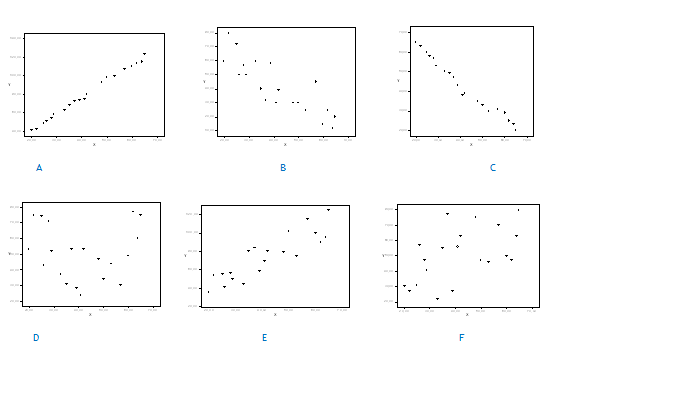
\includegraphics[width=1.10\textwidth]{images/correlaties.png}
	\captionof{figure}{Correlaties}
	\label{fig:correlaties}
%\end{figure}
\end{exercise}

\begin{exercise}
	\label{ex:cats}
	Lees het databestand ``Cats.csv'' in. 
		\begin{enumerate}
		\item Voer een lineaire regressieanalyse uit op de variabelen Lichaamsgewicht (\texttt{Bwt}, afhankelijke variabele) en Gewicht hart (\texttt{Hwt}, onafhankelijke variabele).
		\item Maak een spreidingsdiagram van beide variabelen.
		\item Bereken en teken de regressielijn.
		\item Bereken de correlatie- en de determinatiecoëfficiënt.
		\item Geef een interpretatie van deze resultaten.
	\end{enumerate}
\end{exercise}

\begin{exercise}
  \label{ex:cats-per-geslacht}
	Gebruik dezelfde data als in vorige oefening.
		\begin{enumerate}
		\item Voer een lineaire regressieanalyse uit op de variabelen Lichaamsgewicht (Bwt) en Gewicht hart (Hwt) per geslacht.
		\item Maak een spreidingsdiagram van beide variabelen voor elk van de geslachten.
		\item Bereken en teken telkens de regressielijn.
		\item Bereken de correlatie- en de determinatiecoëfficiënt.
		\item Geef een interpretatie aan deze resultaten.
	\end{enumerate}
\end{exercise}

\begin{exercise}
  \label{ex:pizza}
	Lees het databestand ``Pizza.csv'' in.
		\begin{enumerate}
		\item Voer een volledige lineaire regressieanalyse uit op de variabelen Rating en CostPerSlice. Trek hieruit de juiste conclusies en ga deze ook grafisch na.
		\item Onderzoek een mogelijk verband tussen Rating en Neighbourhood. Welke methode kan je hiervoor gebruiken? Kan je de gegevens van Rating hiervoor in dezelfde vorm gebruiken?
		\item Geef een interpretatie aan deze resultaten.
		\item Stel de kruistabel grafisch voor met een staafdiagram.  Voorzie een legende.
	\end{enumerate}
\end{exercise}

\subsection{Antwoorden op geselecteerde oefeningen}
\label{ssec:analyse-2-variabelen-oplossingen}

\paragraph{Oefening~\ref{ex:muziekwijn-analyse}}

$\chi^2 \approx 18,2792$, Cramér's $V \approx 0,1939$

\paragraph{Oefening~\ref{ex:test-examen}}

\begin{itemize}
  \item $\beta_{0} \approx 0,6333$, $\beta_{1} \approx 0.9667$
  \item $Cov \approx 6,444$, $R \approx 0,9352$, $R^2 \approx 0,8747$
\end{itemize}

\paragraph{Oefening \ref{ex:cats} en \ref{ex:cats-per-geslacht}}

\begin{center}
  \begin{tabular}{lrrrrr}
  	\toprule
    \textbf{Selectie} & \textbf{$\beta_{0}$} & \textbf{$\beta_{1}$} & \textbf{$Cov$} & \textbf{$R$} & \textbf{$R^2$} \\
    \midrule
  	Hele dataset & -0.3511 & 4.0318 & 0.9496 & 0.8041 & 0.6466 \\
  	Female       &  2.9813 & 2.6364 & 0.1979 & 0.5320 & 0.2831 \\
  	Male         & -1.1768 & 4.3098 & 0.9419 & 0.7930 & 0.6289 \\
    \bottomrule
  \end{tabular}
\end{center}
